\section{Auswertung}
\label{sec:Auswertung}

\begin{equation}
  T(t) = \frac{A t^\alpha}{1+Bt^\alpha} + C
\end{equation}

\begin{equation}
  %((A * α * t ** (α - 1) * (1 + B * t ** α)) - (A * t ** α) * (B * α * t ** (α - 1))) / (1 + B * t ** α) ** 2
  \frac{\mathrm{d}T(t)}{\mathrm{d}t} = \frac{αAt^{α - 1} \cdot (1 + B t^α) - A t^α \cdot αBt^{α - 1}}{(1 + B t^ α)^ 2}
\end{equation}

\begin{figure}
  \centering
  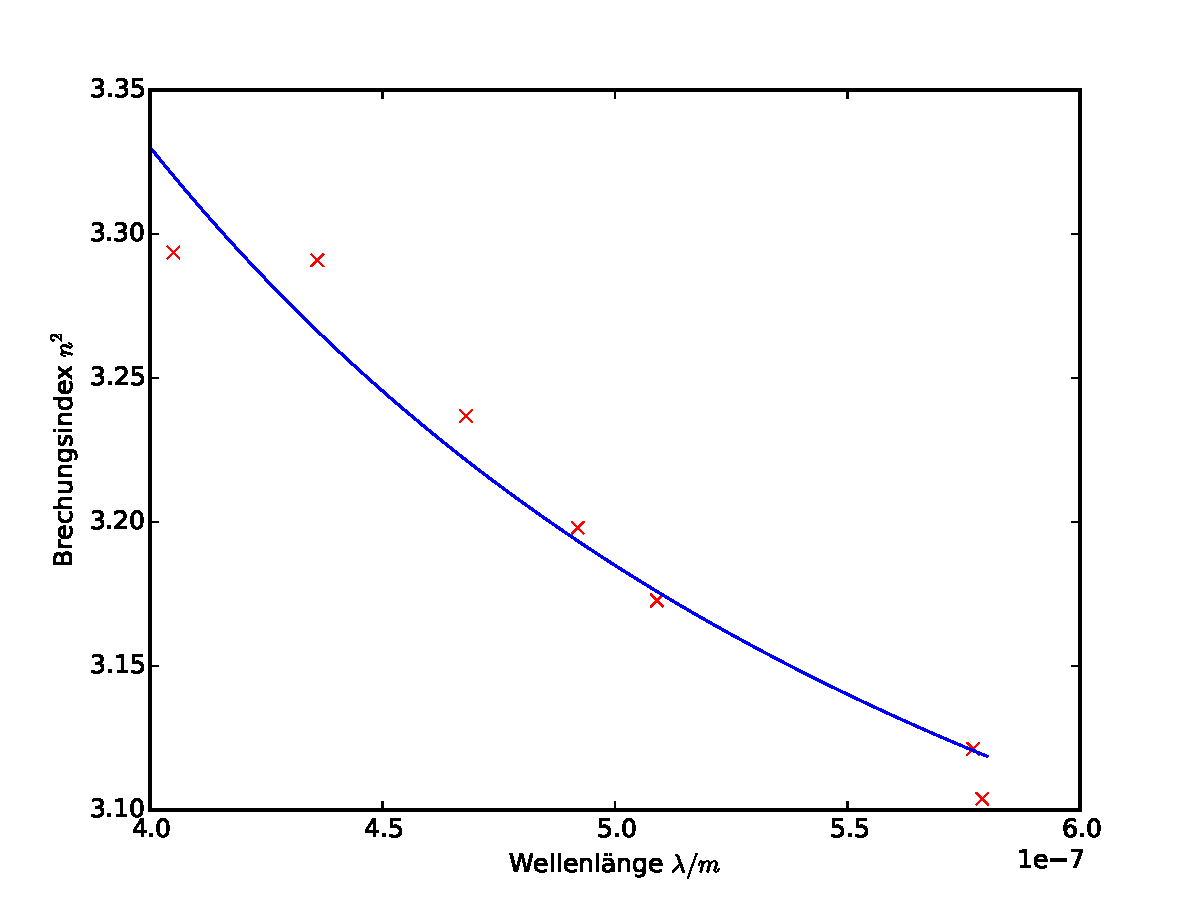
\includegraphics{plot.pdf}
  \caption{Plot des Temperaturverlaufs.}
  \label{fig:temperatur}
\end{figure}

\begin{figure}
  \centering
  \includegraphics{plot_dampfdruck.pdf}
  \caption{Plot der Dampfdruckkurve.}
  \label{fig:dampfdruck}
\end{figure}

\begin{figure}
  \centering
  \input{content/Schema_Wearmepumpe.pdf_tex}
  \caption{Schematischer Aufbau einer Wärmepumpe.}
  \label{fig:wärmepumpe}
\end{figure}

\begin{figure}
  \centering
  \input{content/Aufbau.pdf_tex}
  \caption{Schematischer Aufbau einer Wärmepumpe.}
  \label{fig:aufbau}
\end{figure}

\begin{table}
  \centering
  \caption{Ergebnisse der Auswertung.}
  \label{tab:ergebnisse}
  \sisetup{
    round-mode=places,
    round-precision=3,
  }
  \begin{tabular}{
      l@{}
      S[table-format=4.0]
      S[table-format=1.3] @{${}\pm{}$} S[table-format=1.3]
      S[table-format=2.3] @{${}\pm{}$} S[table-format=1.3]
      S[table-format=2.3] @{${}\pm{}$} S[table-format=1.3]
      S[table-format=3.3] @{${}\pm{}$} S[table-format=2.3]}
    \toprule
    & $t / \si{\second}$
    & \multicolumn{2}{c}{$ν$}
    & \multicolumn{2}{c}{$ν_{\mathrm{ideal}}$}
    & \multicolumn{2}{c}{$\dot m / \si{\gram\per\second}$}
    & \multicolumn{2}{c}{$N / \si{\watt}$} \\
    \midrule
    \input{table.tex}
    \bottomrule
  \end{tabular}
\end{table}

\begin{table}
  \centering
  \caption{Dampfdruckkurve von Dichlordifluormethan.}
  \label{tab:dampfdruck}
  \begin{tabular}{l@{}
      S[table-format=3.2]
      S[table-format=4.0]
    }
    \toprule
    & $T / \si{\kelvin}$
    & $p/ \si{\kilo\pascal}$\\
    \midrule
    \input{table_dampfdruck.tex}
    \bottomrule
  \end{tabular}
\end{table}

\begin{table}
  \scriptsize
  \centering
  \caption{Messdaten.}
  \label{tab:messdaten}
  \begin{tabular}{l@{}
      S[table-format=4.0]
      S[table-format=3.2]
      S[table-format=3.2]
      S[table-format=3.0]
      S[table-format=4.0]
      S[table-format=3.0]
    }
    \toprule
    & $t / \si{\second}$
    & $T_{1} / \si{\kelvin}$
    & $T_{2} / \si{\kelvin}$
    & $p_a / \si{\kilo\pascal}$
    & $p_b / \si{\kilo\pascal}$
    & $P / \si{\watt}$ \\
    \midrule
    \input{table_data.tex}
    \bottomrule
  \end{tabular}
\end{table}
